% Chapter 4

\chapter{Methodology} % Main chapter title

\label{Chapter4} % For referencing the chapter elsewhere, use~\ref{Chapter4} 

In this chapter, we present the methodology of the research. First, we present
the threat model in section~\ref{sec:threat-model}.  After that, we show the
overview of ScaRR algorithm to extract checkpoints and list of actions in
section \ref{sec:overview}. Section~\ref{sec:scarr-checkpoint-marker} discusses
the LLVM implementation to get checkpoints.
Section~\ref{sec:scarr-loa-collector} discusses the methodology of getting list
of actions.  Checkpoints and list of actions are collected to build offline
measurement database that is used for the remote attestation. The last section
shows how to run the LLVM passes to get the result which is presented in
Chapter~\ref{Chapter5}.

\section{Threat Model}
\label{sec:threat-model}

We take the threat model in this research from
ScaRR~\cite{toffaliniScaRRScalableRuntime2019}. There are two parties: attacker
and prover. 

\vspace{0.5cm}
\noindent \textbf{Attacker capabilities:} The attacker aims to control remote
service using various methods such as memory attacks or any attack in
user-space. The attacker has bypassed memory attack protection such as Control
Flow Integrity (CFI) or \( W \bigoplus R \) or ASLR using techniques like
Return-Oriented Programming
(ROP)~\cite{roemerReturnorientedProgrammingSystems2012} or Jump-Oriented
Programming (JOP)~\cite{bletschJumpOrientedProgrammingNew2011}. We do not
consider physical attack and also non-control data attack which does not alter
program's CFG.

\vspace{0.5cm}
\noindent \textbf{Defender capabilities:} The prover uses kernel as trusted
anchor, has common memory corruption attack mitigations such as \( W \bigoplus R
\) and ASLR. Finally, the defender can statically measure the integrity of the
Prover's code (\ie has a hash representation of the prover's code).


\section{Overview}\
\label{sec:overview}

\begin{figure}[t]
    \centerline{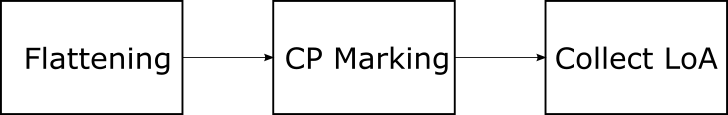
\includegraphics[scale=.75]{Figures/04/scarr-overview.png}}
    \caption{Generating Offline Measurement.}
    \label{fig:scarr-overview}
\end{figure}

The goal of the offline measurement is to get the information to be used in the
remote attestation. In this research, we implement ScaRR Control-flow
model~\cite{toffaliniScaRRScalableRuntime2019} which we present in the
Section~\ref{sec:scarr-model}. 

Figure~\ref{fig:scarr-overview} shows the high-level step on generating the
offline measurement. First, we inline the source code input (which could be in
an intermediate representation form). Section \ref{sec:code-inlining} describes
the inlining process. Next, we mark the checkpoints from inline code,
particularly marking in the basic block of the code. Section
\ref{sec:scarr-checkpoint-marker} discusses this checkpoint marking step. Last,
for each checkpoint, we collect list of actions which indicates how a process
traverses to move from one checkpoint to another. Section
\ref{sec:scarr-loa-collector} talks about the process of getting list of
actions.

\section{Code Inlining}
\label{sec:code-inlining}

\begin{listing}[h]
    \inputminted[
    frame=lines,
    framesep=2mm,
    baselinestretch=1.2,
    fontsize=\footnotesize,
    linenos
    ]{c}{Code/04/factorial.c}
    \caption{Program to calculate factorial.}    
    \label{listing:inlining}
\end{listing}

One most common compiler optimization is inlining. Inlining extracts a body of a
function to the function that calls it. For the context of ScaRR control-flow
model, inlining helps to generate correct checkpoints and list of actions.
Specifically, there is a specific checkpoint called External checkpoint which
appears if there function call instruction in a basic block calls an external
function. Inlining the code reduces most inter-translation-unit function
calls. Hence it makes identifying the checkpoints easier.

In LLVM, we can use an inlining pass that inlines internal function within the same
translation unit.

Consider a program in listing \ref{listing:inlining}. The main function calls
another internal function. Without inlining, the main function control-flow
graph shows no branches and the detail of logic in the factorial function. We
cannot generate accurate offline measurements with this original form. However,
after we inline, we can see branches in the control-flow graph, which represent
the loop in the code. In this inlined representation, we can generate more
accurate offline measurements. Figure \ref{fig:inlining} shows the factorial CFG
without inlining and with inlining.


\begin{figure}[h]
    \centerline{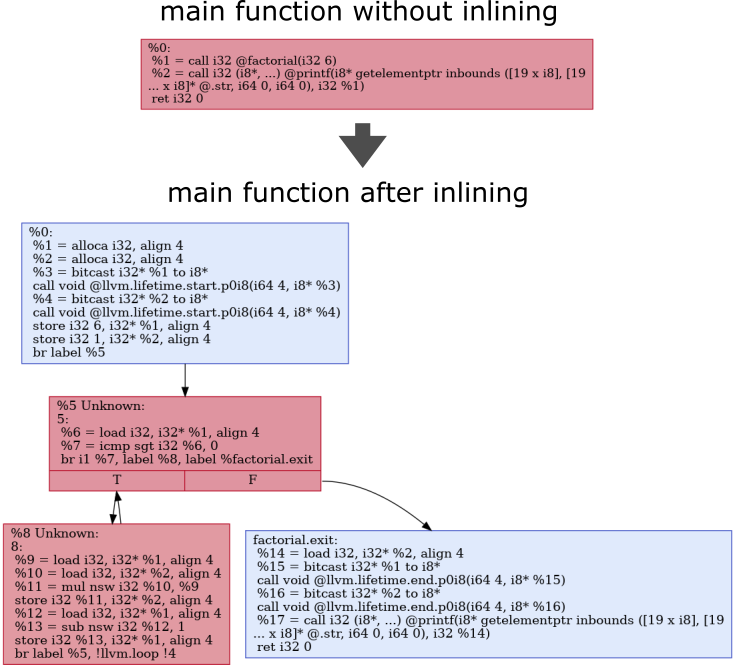
\includegraphics[scale=.80]{Figures/04/inlining-function.png}}
    \caption{Original and Inlined Factorial Program.}
    \label{fig:inlining}
\end{figure}

\section{ScaRR Checkpoint Marker} 
\label{sec:scarr-checkpoint-marker}


Offline measurements use checkpoints and list of actions. We represent offline
measurement as a triplet. The first and second element is checkpoint; the last
element is hashes of the list of actions. The verifier checks the offline
measurement database during remote attestation.

$$(cp_A, cp_B, H(LoA)) \Rightarrow [(BBL_{s1}, BBL_{d1}), ..., (BBL_{sn},
BBL_{dn})]$$

We need program's control-flow graph (CFG) from inlined codes to generate
checkpoints. In Chapter~\ref{Chapter3} we list these four types of checkpoints:
\textbf{Thread Begin}, \textbf{Thread End}, \textbf{Exit Point} and
\textbf{Virtual Checkpoint}. Now we present the heuristic on how we mark it as a
checkpoint when appropriate.  

The logic of the checkpoint marker is to traverse the control flow graph at
least once. We check the basic block checkpoint types as we traverse the basic
blocks. We modify the \texttt{BasicBlock} class to add checkpoint instance variable as
shown in listing~\ref{listing:checkpoint}, so that we can store checkpoint type.

\begin{listing}[htbp]
    \begin{minted}[
        frame=lines,
        framesep=2mm,
        baselinestretch=1.2,
        fontsize=\footnotesize,
        linenos
    ]{c++}
        class BasicBlock ... {
        private:
        // add checkpoint field
            Checkpoint cp;

        public:
            // setter and accessor
        void setCheckpoint(Checkpoint);
        Checkpoint getCheckpoint() const;
        ...
        }
    \end{minted}
    \caption{Add Checkpoint Instance Variable to BasicBlock class.}    
    \label{listing:checkpoint}
\end{listing}

\vspace{0.5cm}
\noindent \textbf{Thread begin} identifies the beginning of a thread or start of
a program. In this thesis, we mark this checkpoint as the first basic block in
the main function. If a program is is a multithreaded program, we mark the
thread begin for each basic block that starts the thread.

\vspace{0.5cm}
\noindent \textbf{Thread end} marks the end of a thread or end of a program. In
a multiple-threaded program, we mark the thread end for each of the basic block
that terminates a thread. In this thesis, we mark thread end checkpoint for the
last basic block that has no more successors.

\vspace{0.5cm}
\noindent \textbf{Exit point} marks that a basic block that calls function
outside of translation unit. The heuristic of marking this type of basic block
is we iterate all instructions in a basic block. We check if the instruction is
a \texttt{call} instruction. Then, we check whether the called function has any
basic block. If the function has no basic block, it means it is an external
function. Hence, we mark this as an exit point and stop. If none of the
instructions is a \texttt{call} instruction or all \texttt{call} instruction in
this basic block call function with nonempty basic block, it means this basic
block calls an internal function. Therefore, this basic block is not an exit
point. Listing~\ref{listing:exit-point-cp} shows the snippet to find ExitPoint.

\begin{listing}[htbp]
    \begin{minted}[
        frame=lines,
        framesep=2mm,
        baselinestretch=1.2,
        fontsize=\footnotesize,
        linenos
    ]{c++}
        for (auto &basicBlock: Function) {
            for (auto &instruction : basicBlock) {
                if (isa<CallInst>(i)) {
                auto *call = &cast<CallBase>(i);
                if (call != nullptr && call->getCalledFunction()->empty()) {
                    // this basicBlock is ExitPoint
                    basicBlock.setCheckpoint(Checkpoint::ExitPoint);
                } 
            }
        } 
    \end{minted}
    \caption{Finding ExitPoint Checkpoint}    
    \label{listing:exit-point-cp}
\end{listing}

\vspace{0.5cm}
\noindent \textbf{Virtual checkpoint} is a checkpoint that marks special cases
such as loop or recursion. We discuss only for loop case in this thesis.
Virtual checkpoint in a loop is a loop header. The heuristic to find a loop
header is to use \texttt{DominatorTree} to find a loop. After we find a loop,
then we just need to get the header. Although there is no direct API to check
whether a basic block is a loop header, LLVM provides it in LoopInfoBase API.
See Listing~\ref{listing:virtual-cp}

\begin{listing}[htbp]
    \begin{minted}[
        frame=lines,
        framesep=2mm,
        baselinestretch=1.2,
        fontsize=\footnotesize,
        linenos
    ]{c++}
    void findVirtualCheckpoint(DominatorTree &DT, Function &F) {
        DT.recalculate(F);
        // generate the LoopInfoBase for the current function
        LoopInfoBase<BasicBlock, Loop>* KLoop = new LoopInfoBase<BasicBlock, Loop>();
        KLoop->releaseMemory();
        KLoop->analyze(DT);
        for (auto &bb : F) {
            // Since the BasicBlock would have been inlined, 
            // just traverse from main function
            if (F.getName() == "main") {
                auto loop = KLoop->getLoopFor(&bb);
                if (loop != nullptr) {
                    // found VirtualCheckpoint
                    loop->getHeader()->setCheckpoint(Checkpoint::Virtual);
                }
            }
        }
    }
    \end{minted}
    \caption{Getting Virtual Checkpoint}
    \label{listing:virtual-cp}
\end{listing}




\section{ScaRR LoA Collector}
\label{sec:scarr-loa-collector}

Checkpoints information is a requirement to get the list of actions.  We
traverse the paths between two checkpoints and add significant basic blocks that
direct the path between the two checkpoints. Those basic blocks comprise the
list of actions. 

\begin{listing}[t]
    \begin{minted}[
        frame=lines,
        framesep=2mm,
        baselinestretch=1.2,
        fontsize=\footnotesize,
        linenos
    ]{c++}
    function collectLoaRecursive(firstCheckpoint, successorBasicBlock) {
        if (firstCheckpoint has more than one successor and 
            no LoA is added yet) {
                add firstCheckpoint as 1st (cpA) LoA for this path
        }
        
        for (succ = successors of successorBasicBlock) {
            if (succ is a checkpoint) {
                if (one LoA has been added for this path) {
                    add succ as the 2nd (cpB) LoA
                }
                add cpA and cpB LoA to measurement
            } else if (succ is not a checkpoint) {
                if (LoA is non empty and the previous LoA is a checkpoint) {
                    add succ as the 2nd LoA
                }
                recursively collectLoaRecursive(firstCheckpoint, succ)
            }
        }
    }

    function collectLoa(list of basicBlock) {
        for (basicBlock = all basicBlocks) {
            collectLoaRecursive(basicBlock, basicBlock)
        }
    }
    \end{minted}
    \caption{Pseudocode to Collect List of Actions.}
    \label{listing:loa-pseudocode}
\end{listing}

The algorithm of getting LoA between two checkpoints is a little bit more
complex. First, we iterate all the basic blocks. Once we find a basic block with
some checkpoint types, we mark this as $cpA$. Next, we recursively traverse the
successor of $cpA$ until we find another checkpoint $cpB$. It is possible for
$cpA = cpB$. If there is no branch between the two checkpoints, the LoA is an
empty set. If there is a branch, the first LoA is always $cpA$ and the second
LoA is always be the first basic block after the branch \textemdash{} which can
be $cpB$ or just a non-checkpoint basic block. We show the pseudocode for this
logic in listing \ref{listing:loa-pseudocode}.  Interested readers can refer to
the source code of this pass to see the detail.
